% !TeX root = ../main.tex

\section{Problem Definition}
    \frame{\sectionpage}

    \begin{frame}{Seat Planning with Social Distancing}
      \begin{itemize}
      \item Group type $\mathcal{M} = \{1, \ldots, M\}$.
      \item Row $\mathcal{N} = \{1, \ldots, N\}$.
      \item The social distancing: $\delta$ seat(s).
      \item $n_i = i + \delta$: the new size of group type $i$ for each $i \in \mathcal{M}$.
      \item The number of seats in row $j$: $S_j, j \in \mathcal{N}$.
      \item $L_j = S_j + \delta$: the length of row $j$ for each $j \in \mathcal{N}$.
      \end{itemize}
      
      \begin{figure}[ht]
        \centering
        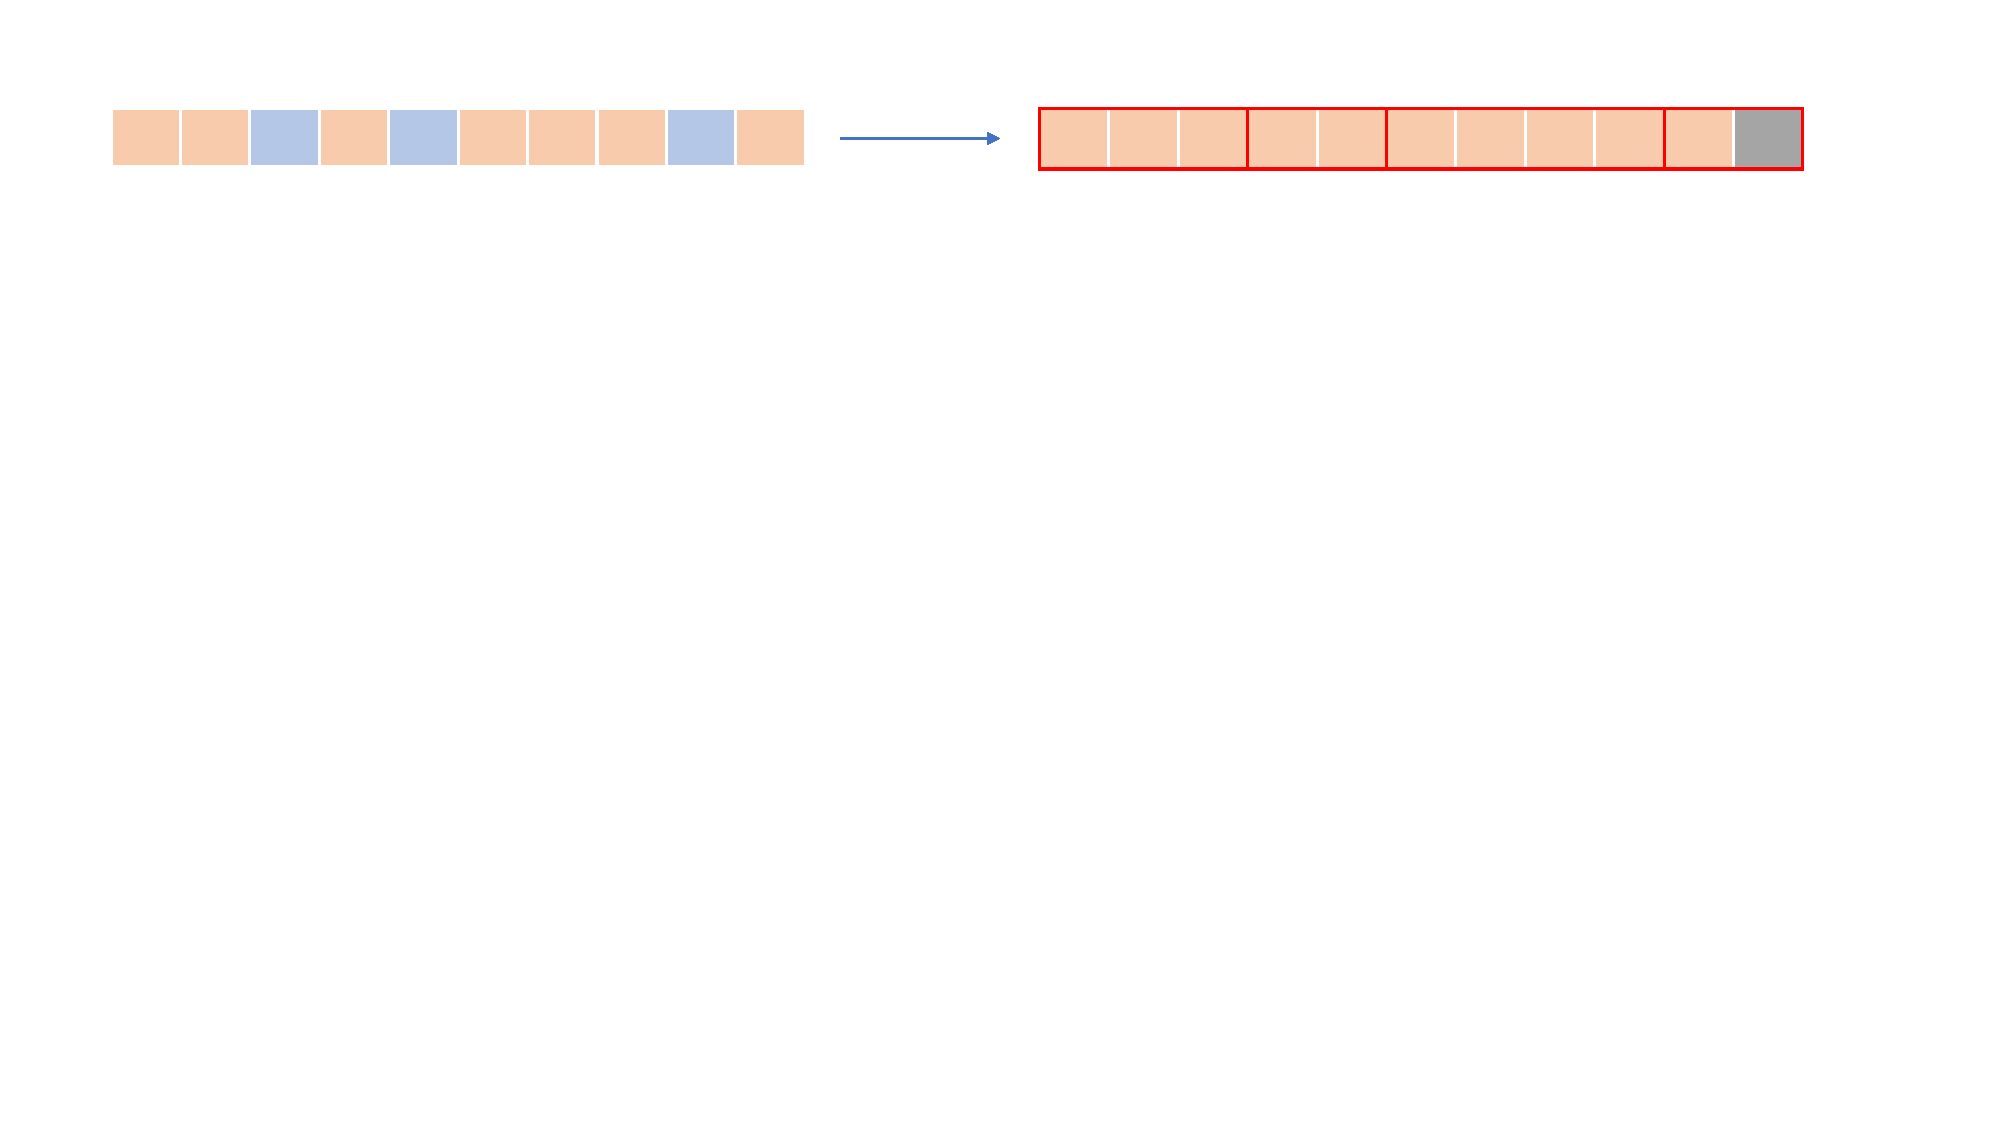
\includegraphics[width = 0.8\textwidth]{./images/dummy_seat.pdf}
        \caption{Problem Conversion with One Seat as Social Distancing}
    \end{figure}
    \end{frame}

  \begin{frame}{Basic Concepts}
    \begin{itemize}
      \item $P_{k} = (t_1, \ldots, t_M)$, pattern, the seat planning for each group type $i, i \in \mathcal{M}$ in one row.
      \item For each pattern $k$, $a_k, b_k$ indicate the number of groups and the unused seats, respectively.
      \item Loss for pattern $k$: $a_k \delta + b_k - \delta$.
      \item Largest patterns: Minimal loss with fixed length $L$. 
      \item Full patterns: $b_k =0$.
      \item[-] {\color{blue} Example}: 
      
      $\delta = 1$, $M =4$, $n_1 = 2, n_2 = 3, n_3 = 4, n_4 = 5$, $L = 21$.
      
      Largest patterns: $(0, 0, 0, 4), (0, 0, 4, 1), (0, 2, 0, 3)$.
      
      Not a Full pattern: $(0, 0, 0, 4)$.
    \end{itemize}
  \end{frame}

  \begin{frame}{Dynamic Seat Assignment Problem}
    \centering
    \small
    \begin{itemize}
    \item[-] There is one and only one group arrival at each period, $t = 1, \ldots, T+1$. 
    \item[-] The probability of an arrival of group type $i$: $p_i$.  
    \item[-] $\mathbf{L} = (l_1, l_2, \ldots, l_{N})$, where $l_j =0,\ldots, L_j, j\in \mathcal{N}$: Remaining capacity.
    \item[-] $u_{i,j}$: Decision. Assign group type $i$ to row $j$, $u_{i,j} =1$.
    \item[-] $\mathbf{e}_j^{\top}$: Unit row vector with $j$-th element being 1.
    \item[-] $V_{t}(\mathbf{L})$: Value function at period $t$, given remaining capacity, $\mathbf{L}$.
    \end{itemize}

    $$V_{t}(\mathbf{L}) = \max_{u \in U(\mathbf{L})}\{ \sum_{i=1}^{M} p_i ( \sum_{j=1}^{N} i u_{i,j} + V_{t+1}(\mathbf{L}- \sum_{j=1}^{N} n_i u_{i,j}\mathbf{e}_j^{\top} ))\}$$

    \small
    \begin{itemize}
      \item[-] DP is computationally complex caused by the curse of dimensionality.
      \item[-] We give a seat planning by stochastic programming firstly, then apply stochastic planning policy to make the decision.
    \end{itemize}
\end{frame}